% set font and paper size
\documentclass[11pt,a4paper]{article}

% change to german
\usepackage[german]{babel}

% better hyphenation
\usepackage[final]{microtype}
\usepackage{csquotes}

% packages, images, math
\usepackage{geometry, graphicx, amsmath, amsfonts, array, multicol, multirow}

% bar charts
\usepackage{bchart}

% check for unused references, not working
% \usepackage{refcheck}

% for bibliography
\usepackage[
    backend=biber,
    style=alphabetic,
    sorting=ynt,
    minalphanames=3,
]{biblatex}
\addbibresource{./references.bib}


% import line spacing
\usepackage{setspace}

% colors
\usepackage{xcolor}

% for urls
% break urls on line end
\usepackage[breaklinks, colorlinks=true, urlcolor=blue, citecolor=blue, linkcolor=black]{hyperref}

% Remove Indentation at new line
\setlength{\parindent}{0cm}

% Set Font to Arial, needs xelatex
\usepackage{unicode-math}
\usepackage{fontspec}
\setmainfont{Arial}

% Set Font to Helvet
% \usepackage{helvet}
% \renewcommand{\familydefault}{\sfdefault}

% Set Layout
\geometry{
    a4paper,
    left=25mm,
    right=25mm,
    top=25mm,
    bottom=20mm
}

% set line spacing
\setstretch{1.5}

% document
\begin{document}

\addtocounter{page}{-2}

% deckblatt

% content
\title{Supersonic Algorithms}
\author{Anton Rodenwald (18)}

\maketitle

\thispagestyle{empty}

\large\begin{tabular}{l p{12cm}}

    Projektbetreuerin: & Birgit Ziegenmeyer                                                  \\

    Institution:       & Schillerschule Hannover                                             \\

    Thema des Projektes:
                       & Implementation von Algorithmen in verschiedenen Programmiersprachen
    und Analyse dieser in Bezug auf die besten Techniken zur Optimierung,
    um die Umsetzung hochperformanter und effizienter Programme zu erforschen.               \\

    Fachgebiet:        & Mathematik/Informatik                                               \\

    Wettbewerbssparte: & Jugend forscht                                                      \\

    Bundesland:        & Niedersachsen                                                       \\

    Wettbewerbsjahr:   & 2023                                                                \\
\end{tabular}


\clearpage

% kurzfassung

\thispagestyle{empty}

\section*{Kurzfassung}

Durch den Informatikunterricht bekam ich die Idee zu erforschen, wie sich
die Implementation von Algorithmen optimieren lässt.
Relevanz hat die Optimierung der Implementation, weil sich durch effiziente Programme Zeit, Geld
und z. B. in Rechenzentren auch Strom sparen lässt.
Einen besonderen Fokus legte ich dabei auf die Sprache Python im Vergleich mit C/C++.
Meine Erwartung war, das Python Implementationen deutlich langsamer sein würden als C/C++,
was sich mit Aussagen auf Programmier-Foren deckte, die ich mir angeschaut hatte.
Ich nutzte den Sortieralgorithmus Quicksort als Beispiel und implementierte viele optimierte Versionen
in Python unter Nutzung der Bibliotheken NumPy, Numba, Cython und CTypes.
Nach Messung der Ausführungszeit konnte ich feststellen, dass Python mit NumPy und Numba
so schnell wie C++ werden kann.
Außerdem fiel mir auf, wie stark das Zusammenspiel zwischen Python und C/C++ ist
und wie sich interpretierte und kompilierte Programmiersprachen unterscheiden.

\clearpage

\renewcommand*\contentsname{Inhaltsverzeichnis}

\tableofcontents

\clearpage

\section{Einleitung}

In meinem Projekt wollte ich herausfinden, wie sich Programme durch geschickte Implementation
in ihrer Ausführung beschleunigen lassen. Ich fragte mich, welche Optimierungen den größten Zuwachs
an Performance bringen. Diese Frage schien mir relevant, da durch effiziente Programme Zeit, Geld
und Strom z. B. in Rechenzentren gespart werden können.
Es ging ausdrücklich nicht darum, verschiedene Algorithmen auf theoretischer Ebene
miteinander zu vergleichen, da dies bereits zu Genüge gemacht wurde \cite{sortieralgorithmenwikipedia}.
Die Idee entstand dadurch, dass ich im Herbst 2022 im Informatikunterricht
Sortieralgorithmen wie den von Hoare entwickelten Quicksort-Algorithmus kennenlernte \cite{quicksortwikipedia}.
Ich stellte mir die Frage, wie man eine Liste von 10 Millionen zufällig generierten positiven Ganzzahlen
am schnellsten sortieren kann. Da algorithmisch bei Quicksort keine Verbesserung möglich schien,
kam ich so auf das Thema, die Ausführung möglichst zu beschleunigen, indem ich mich mit
Implementationsoptimierungen beschäftigte. Dabei wollte ich auch ergründen, wodurch sich Unterschiede
in der Performance zwischen Programmiersprachen erklären lassen. Meine Hypothese war dabei,
dass C/C++ deutlich schneller als andere Sprachen wie z. B. Python sein würde und dass
ich in Python die Performance nicht so stark optimieren kann.  Als Programmierer bemühte ich
nun das Internet und fand vier Quellen, die C/C++ als 10x bis 100x mal schneller beschrieben,
was sich mit meiner Vermutung deckte \cite{pyengineeringvscpp} \cite{quorepythonvscpp}
\cite{stopythonvscpp}.
Auch fand ich einige Artikel von eifrigen Programmierern, die sich mit der Optimierung
von Python beschäftigten. Ich wurde so zur Nutzung von Cython, CTypes, Numba und NumPy bewegt,
wovon die letzteren beiden mir bereits bekannt waren \cite{cythonctypes}.
Meine Internetsuche nach den besten Optimierungen für Python ergab nur Tipps, aber keine
guten Vergleiche der Geschwindigkeit, weshalb ich entschied, dass ein Vergleich der
Optimierungsmöglichkeiten sinnvoll sein könnte.
\cite{pythonopt1} \cite{pythonopt2} \cite{pythonopt3}.

\section{Materialien, Vorgehen, Methode}

\subsection{Materialien}
Für mein Projekt nutzte ich meinen Desktop PC (Linux) zum Implementieren und Ausführen der Programme.
In diesem verbaut sind als CPU der Ryzen 7 2700 und 16 GB Arbeitsspeicher. Außerdem nutzte ich mehrere Programme.
Neben Visual Studio Code (Implementierung der Programme) und \LaTeX (Erstellen der schriftlichen Arbeit)
waren dies die Compiler oder Interpreter zum Ausführen der verschiedenen Programmiersprachen.
Diese Programme waren (mit Versionsangabe) Clang++ 14.0.6 (C/C++ Compiler), Python 3.10.8 (Ausführen von Python Programmen),
Java 19.0.1 (Kompilieren und Ausführen von Java), Lua 5.4.4 (Ausführen von Lua Programmen),
Nodejs 18.8.0 (Ausführen von Javascript Programmen), Julia 1.8.3 (Ausführen von Julia Programmen)
und Go 1.19.4 (Go Compiler).

\subsection{Vorgehen und Methode}

Mein Vorgehen war für alle getesteten Programmiersprachen ähnlich.
Zuerst generierte ich in der jeweiligen Sprache eine unsortierte Liste bzw. ein Array mit 10 Millionen Pseudo-Zufallszahlen,
die anschließend von einer Quicksort Implementation in dieser Sprache aufsteigend sortiert wurden.
Da jede Sprache über Möglichkeiten der Zeitnahme verfügt, konnte ich so die zur Sortierung benötigte Zeit
ermitteln. In Python implementierte ich dazu eine Timer-Klasse
(Abb. 1). Diese konnte ich im Quellcode nutzen, um die Zeit von Programmcodeabschnitten zu messen (Abb .2).
Die Ergebnisse dieser Messungen ließ ich mir auf der Konsole ausgeben (Abb. 3).

\begin{center}
    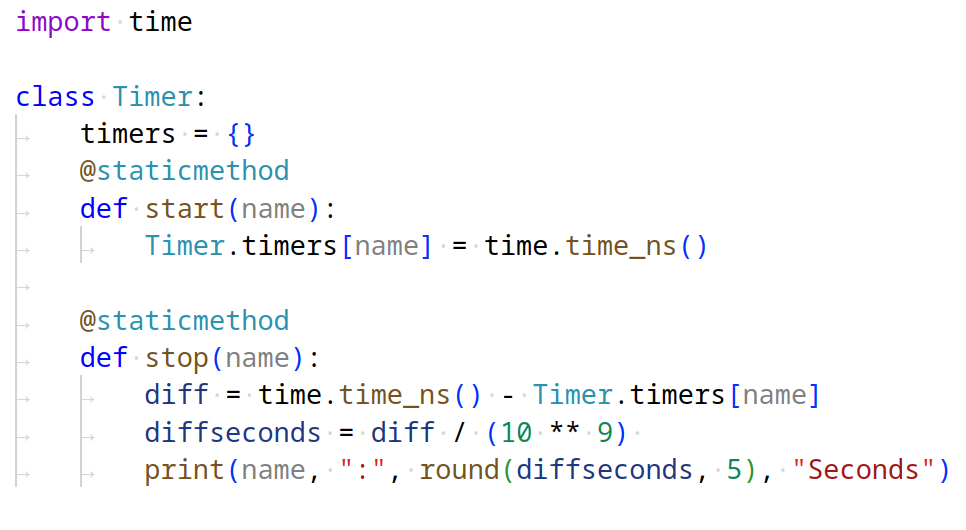
\includegraphics[width=0.75\textwidth]{screenshots/pythontimerlight.png}

    Abb. 1 Timer Klasse
\end{center}

\begin{center}
    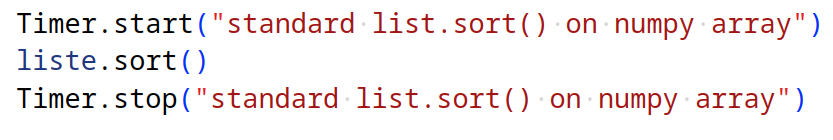
\includegraphics[width=.75\textwidth]{screenshots/timerexamplelight.png}

    Abb. 2 Zeitnahme

    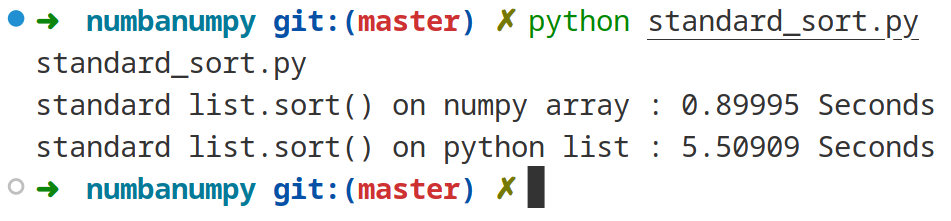
\includegraphics[width=.75\textwidth]{screenshots/outputexamplelight.png}

    Abb. 3 Beispielausgabe
\end{center}


In den Sprachen Lua, Java, Javascript, Julia, Go und C/C++ nahm ich dabei keine weiteren Optimierungen vor,
sondern fokussierte mich voll und ganz auf die Optimierung von Python.
Ich nutzte dabei die Bibliotheken NumPy, Numba, CTypes und Cython, über die ich mich, nach Programmierer
Manier, durch das Nutzen einer nicht auflistbaren Anzahl an Online-Ressourcen und
durch das Lesen der Dokumentationen informierte \cite{cythondocs} \cite{cythondocsnumpy} \cite{cythonctypes}.
Eine Schwierigkeit dabei war, dass ich kaum Erfahrung mit diesen Python-Bibliotheken hatte.
In Python entwickelte ich dann eine Vielzahl an verschiedenen Funktionen zur Generierung von Zufallszahlen
und implementierte auch viele verschiedene Versionen von Quicksort. Dabei kombinierte ich die
genannten Bibliotheken und Python Standard-Funktionen, um neue Variationen zu schaffen,
die potenziell bessere Performance bieten.
Ich probierte dabei einfach herum nach dem \textit{Trial and Error} Prinzip und schaute, was
die Performance erhöhte.
Meine Versionen waren somit Weiterführungen der Ansätze aus diesen Bibliotheken, aus denen ich
verschiedene Optimierungsmöglichkeiten nutzte.
Ein Beispiel sind die Bibliotheken Numba und NumPy. Beide brachten meinen Versionen einen
Geschwindigkeitsboost, doch durch die Kombination beider wurde die Zeitersparnis noch größer.
Jede dieser Versionen führte ich nun mehrmals aus und nahm die beste Zeit.
So hatte ich nun für jede Version eine Ausführungsdauer.
Wichtig dabei war, alle Tests auf dem gleichen Computer zu machen,
da sich bei unterschiedlicher Hardware
die Ergebnisse unterscheiden. Diese wären sonst nicht vergleichbar gewesen.
Am Ende des Projektes implementierte ich außerdem noch den Radixsort-Sortieralgorithmus in C++ mithilfe
einiger Internetquellen um herauszufinden, was die schnellste Möglichkeit zur Sortierung von 10 Millionen
Zahlen ist \cite{terdiman} \cite{michael} \cite{intelavxdocs} \cite{avxguide}.
Dabei muss gesagt sein, dass Radixsort ein anderer
Algorithmus ist und somit nicht mit den anderen Programmen mit Quicksort vergleichbar ist.

\subsection{Schwierigkeiten}

Die größte Schwierigkeit war, dass ich auf diesem Themengebiet noch nicht sehr viel Vorerfahrung hatte.
Außerdem waren die Konzepte teils komplex und es war nicht immer einfach, im Internet gute Beispiele
zu finden. Vor dem Projekt hatte ich mich z. B. noch nie mit der Python Bibliothek CTypes beschäftigt
und deshalb fand ich meist erst nach längerem Suchen im Internet eine Lösung für auftretende Fehler.
Auch bei der Implementation von Programmen in C++ hatte ich teils meine Schwierigkeiten, da das Verstehen
von einigen Bitoperationen erstmal ein Eindenken in die Thematik erforderte.
Ein für mich nicht lösbares Problem war auch die Implementierung in Go.
Dort war das Sortieren von mehr als 7 Millionen Zahlen mit einer rekursiven Quicksort leider nicht möglich.
Ich fand heraus, dass dies an der Implementierung von Rekursion in Go liegt, die viel Arbeitsspeicher
verbraucht, was ein Problem war, da der Arbeitsspeicher für eine Funktion auf 1 Gigabyte begrenzt ist.
Diese Grenze wurde ungünstigerweise dann erreicht, wodurch das Programm abstürzte.
\cite{godeeprecursions} \cite{goroutinesize}.

\section{Ergebnisse}

\subsection{Generierung von 10 Millionen zufälligen Zahlen in Python}

\begin{bchart}[min=0, max=30, scale=1.9]
    \bcbar[label=1, text=List Comprehension Python mit Konvertierung zu numba.typed list]{26.849}
    \smallskip
    \bcbar[label=2, text=\hspace{7cm}List Comprehension Python]{9.307}
    \smallskip
    \bcbar[label=3, text=\hspace{2cm}List Comprehension Python mit Numba]{1.148}
    \smallskip
    \bcbar[label=4, text=\hspace{2cm}NumPy np.random.randint mit Numba]{0.401}
    \smallskip
    \bcbar[label=5, text=\hspace{2cm}NumPy np.random.randint]{0.051}
    \smallskip
    \bcxlabel{\bf{Ausführungszeit in Sekunden}}
\end{bchart}

\vspace{0.5cm}


Wie im Vorgehen beschrieben generierte ich unsortierte Listen von Zufallszahlen,
damit ich testen konnte, wie schnell meine Quicksort Implementationen diese
sortierten. Die Version mit List Comprehensions in Python (2) dauerte relativ lange.
Dies war ein Hindernis beim Entwickeln und Testen der eigentlichen Quicksort Implementationen,
da so jeder Test des Programms während dem Entwickeln länger dauert.
Deshalb optimierte ich die Generierung mit Numba (3, 4) und NumPy (4, 5).
Es zeigte sich, dass alle 3 optimierten Versionen deutlich schneller waren.
Dies entsprach meinen Erwartungen, dass die Bibliotheken mehr Performance bringen.
Auffallend war dabei, dass die Kombination von NumPy und Numba langsamer war,
als NumPy allein.
Am längsten dauerte die Generierung mit List Comprehensions und anschließender
Konvertierung zu einer typisierten Numba Liste (5). Diese Version entwickelte
ich allerdings nur, weil eine Optimierung der Quicksort mit Numba nicht mit normalen Python-Listen
kompatibel war. Für Numba müssen die Listen nämlich in einem kompatiblen Format vorliegen,
weshalb die Konvertierung nötig war.

\subsection{Quicksort Implementationen in Python mit verschiedenen Optimierungen und Vergleich mit C++}

\begin{bchart}[min=0, max=80, scale=1.9]
    \bcbar[label=1, text=Quicksort mit NumPy Array]{72.231}
    \smallskip
    \bcbar[label=2, text=Quicksort mit Cython kompiliert]{52.808}
    \smallskip
    \bcbar[label=3, text=Quicksort mit Python Liste]{40.493}
    \smallskip
    \bcbar[label=4, text=\hspace{5cm}Quicksort mit Cython (alle Optimierungen)]{14.717}
    \smallskip
    \bcbar[label=5, text=\hspace{5cm}Quicksort mit Cython (statische Typisierung)]{14.403}
    \smallskip
    \bcbar[label=6, text=\hspace{5cm}Quicksort mit Numba und numba.typed list]{9.744}
    \smallskip
    \bcbar[label=7, text=\hspace{5cm}list.sort() mit Python Liste]{5.314}
    \smallskip
    \bcbar[label=8, text=\hspace{5cm}Quicksort mit Numba und NumPy Array]{1.805}
    \smallskip
    \bcbar[label=9, text=\hspace{5cm}C++ Quicksort]{1.051}
    \smallskip
    \bcbar[label=10, text=\hspace{5cm}C Quicksort aufgerufen mit CTypes]{1.035}
    \smallskip
    \bcbar[label=11, text=\hspace{5cm}C++ Standard Quicksort (std::sort)]{0.909}
    \smallskip
    \bcbar[label=12, text=\hspace{5cm}list.sort() mit NumPy Array]{0.894}
    \smallskip
    \bcxlabel{\bf{Ausführungszeit in Sekunden}}
\end{bchart}

In diesem Diagramm sind meine verschiedenen Versionen der Quicksort in Python,
die standardmäßig verfügbaren Sortierfunktionen von Python und C++
sowie eine in C++ implementierte Quicksort zu sehen.
Alle diese Versionen ließ ich eine vorher generierte, unsortierte Liste aus
10 Millionen zufälligen Zahlen sortieren.
Meine im Informatikunterricht entwickelte Version (3) brauchte ca. 41 Sekunden
zur Sortierung. Überraschend war für mich dann, dass Versionen mit Cython und NumPy
(1, 2) teils länger brauchten. Dies hatte ich nicht erwartet. Ich ging eigentlich davon aus,
dass es nur positive Veränderungen geben würde, also meine Implementationen nur schneller werden
würden. Als ich dann Cython zur statischen Typisierung nutzte, zeigte sich ein
guter Zuwachs an Performance (5). Weitere Optimierungen mit Cython (4)
schienen aber keinen Effekt zu haben, was mich wunderte.
Da Cython vor der Ausführung kompiliert wird, hatte ich eigentlich mit einer
größeren Geschwindigkeitserhöhung gerechnet, was nicht der Fall war.
Ungefähr 4.5x schneller war meine Version mit Numba und der Numba Typed List (6).
Nutzte ich Numba nun in Kombination mit einem NumPy Array (8), so erhöhte sich
die Geschwindigkeit nochmal um ein Vielfaches.
Meine Version mit Numba und NumPy (8) war sogar schneller als die normale
Sortierfunktion für Python Listen (7). Dies bestätigte meine Erwartungen,
dass NumPy und Numba einen großen Boost in Performance bringen,
doch es überraschte mich, dass dieser so groß war.
Einzig schneller waren nur einige C/C++ Versionen (9, 10, 11) und die
standardmäßige Sortierfunktion für NumPy Arrays, was ich so erwartet hatte.
Meine in C++ implementierte Quicksort (9) war dabei ähnlich schnell
wie die standardmäßige C++ Sortierfunktion (11).
Wichtig zu erwähnen zur Version mit CTypes (10) ist, dass die Konvertierung
einer Python Liste in ein für C verständliches Format auch nochmal ca. 2 Sekunden
Zeit kostete.
Es zeigt sich, dass NumPy eine genauso schnelle Sortierung wie C++ ermöglicht.
Dies überraschte mich sehr, weil es meiner Hypothese und den Foren-Beiträgen,
die ich gelesen hatte, komplett widersprach.
Ich fragte mich, wie sich die Versionen 3 und 12 unterschieden.
Um mir diese Frage zu beantworten stellte ich einige Überlegungen an,
die ich später diskutieren werde.

\subsection{Quicksort Implementationen in weiteren Sprachen im Vergleich}

\begin{bchart}[min=0, max=15, scale=1.9]
    \bcbar[label=1, text=Quicksort Lua]{11.528}
    \smallskip
    \bcbar[label=2, text=Lua table.sort (Standardsortierung)]{11.035}
    \smallskip
    \bcbar[label=3, text=\hspace{7cm}Java Collection.sort (Standardsortierung)]{5.016}
    \smallskip
    \bcbar[label=4, text=\hspace{7cm}Quicksort Javascript]{3.167}
    \smallskip
    \bcbar[label=5, text=\hspace{7cm}Quicksort Java]{2.828}
    \smallskip
    \bcbar[label=6, text=\hspace{7cm}Quicksort Julia und Julia sort (Standardsortierung)]{1.374}
    \smallskip
    \bcbar[label=7, text=\hspace{7cm}Javascript array.sort (Standardsortierung)]{1.159}
    \smallskip
    \bcbar[label=8, text=\hspace{7cm}Quicksort Go (7 Millionen Zahlen)]{0.919}
    \smallskip
    \bcxlabel{\bf{Ausführungszeit in Sekunden}}
\end{bchart}

Neben C++ und Python interessierte mich auch, wie schnell das Sortieren mit
einer Implementation der Quicksort in anderen Sprachen möglich ist.
Ich nahm dabei aufgrund meines limitierten Wissens in diesen Sprachen keine Optimierungen
vor. Dies tat ich auch, weil mich interessierte, wie schnell die nativen
Implementationen der Quicksort in diesen ist.
Es fällt direkt auf, dass Lua (1, 2) sowohl mit der Quicksort als auch mit der
standardmäßigen Sortierung im Vergleich sehr schlecht abschneidet.
Darauf folgt die standardmäßige Sortierung in Java (3).
Diese ist überraschenderweise langsamer als meine Quicksort Implementation in Java (5).
Zwischen diesen beiden liegt meine Quicksort in Javascript.
Darauf folgt dann Julia (6), wo meine eigene Quicksort fast genauso schnell war wie
die standardmäßige Sortierfunktion.
Einzig schneller sind nur die standardmäßige Sortierfunktion in Javascript (7) und meine
Quicksort Implementation in Go (8). Diese ist allerdings nur bedingt vergleichbar, da ich
aufgrund von beschriebenen Schwierigkeiten nur 7 Millionen Zahlen sortieren konnte.
Meine Go-Variante lässt sich also nicht als schnellste Version bezeichnen.


\subsection{C++ Radixsort Implementationen}

\begin{bchart}[min=0, max=2.5, scale=1.9]
    \bcbar[label=1, text=Radixsort mit Basis 10 (Countingsort)]{2.269}
    \smallskip
    \bcbar[label=2, text=\hspace{3cm}Radixsort mit Basis 256 (Bytesort)]{0.244}
    \smallskip
    \bcbar[label=3, text=\hspace{3cm}Radixsort mit Basis 256 (Bytesort) und AVX2]{0.240}
    \smallskip
    \bcxlabel{\bf{Ausführungszeit in Sekunden}}
\end{bchart}

In den vorigen Teilen ging es um die Optimierung der Quicksort. Dieser Abschnitt
behandelt die Radixsort, ist also nicht mit den Ergebnissen und Überlegungen von davor vergleichbar.
Es wurden hier nicht nur Optimierungen, sondern auch andere Algorithmen genutzt.
Der Grund warum ich mich auch mit der Radixsort beschäftigte ist, dass ich
den schnellsten Weg zur Sortierung von 10 Millionen Zufallszahlen finden wollte.
Die Quicksort hat eine durchschnittliche Komplexität von \boldmath$O(n\log n)$,
die Radixsort von \boldmath$O(n \cdot w)$. Die Radixsort ist also algorithmisch gesehen schneller.
Meine erste Implementation der Radixsort (1) brauchte 2.269 Sekunden. Sie war damit
also langsamer als viele der Versionen der Quicksort aus den vorigen Diagrammen.
Meine weiteren Implementationen (2, 3) mithilfe der Artikel von Pierre Terdimann und
Michael Herf waren dann allerdings deutlich schneller als alle Vorigen der Quicksort Versionen
\cite{terdiman} \cite{michael}.
Dies zeigte mir, dass die korrekte Implementation von Algorithmen eine Rolle spielt,
da meine erste Version zwar einen überlegenden Algorithmus nutzte, aber trotzdem
langsamer war. Auch zeigte sich, dass bei korrekter Implementation die Wahl des
Algorithmus sehr wichtig ist. Bei meinen besten Versionen der Radixsort und der Quicksort
war erstere deutlich schneller. Daraus schloss ich, dass vor der Optimierung der
Implementation am besten erst der beste bekannte Algorithmus gewählt werden sollte.
Ich fragte mich, wieso die Radixsort nicht häufiger benutzt wird, was ich mir leider nicht
beantworten konnte.

\clearpage

\section{Ergebnisdiskussion}

\subsection{Erklärung der Ergebnisse}

Zwischen den verschiedenen Implementationen gab es große Unterschiede in Bezug auf die
Ausführungsgeschwindigkeit. Wie diese zustande kamen, will ich im Folgenden erklären.
Dazu ist es wichtig, dass Konzept von interpretierten und kompilierten
Programmiersprachen zu verstehen. Bei einer interpretierten Programmiersprache wie
Python wird der Quellcode von einem speziellen Programm, dem Interpreter, zur Zeit der Ausführung verarbeitet.
Dabei müssen viele Prüfungen durchgeführt werden, damit das Programm richtig ausgeführt werden kann.
Bei kompilierten Sprachen hingegen werden alle Prüfungen vor dem Ausführen durchgeführt.
Jeder Quellcode in diesen Sprachen muss vor der Ausführung kompiliert werden und in
Maschinensprache umgewandelt werden. Im Gegensatz zur Interpretation können dabei auch deutlich
mehr automatische Optimierungen vom Compiler vorgenommen werden.
Deswegen sind kompilierte Sprachen generell nahezu immer schneller als interpretierte.
Die Bibliotheken NumPy, CTypes, Numba und Cython basieren darauf, dass weniger Python-Quellcode
interpretiert werden muss. Dies geschieht dadurch, dass diese Möglichkeiten zur
Nutzung von kompiliertem Code in Python bieten.
Dabei geht jede Bibliothek unterschiedlich vor.
NumPy, CTypes und Python-Standardfunktionen bieten Python Zugriff auf schnelle und
bereits kompilierte C Funktionen.
Numba ermöglicht die Just-in-Time Kompilierung, also bestimmte Teile des Python Quellcodes
während der Ausführung für bessere Performance zu kompilieren.
Cython ermöglicht diese Kompilierung bereits vor der Ausführung in gewissem Maße.
All diese Konzepte bringen Python näher an die kompilierten Sprachen heran, und somit
auch an die Geschwindigkeit von C/C++. Ich erfuhr dies durch ein Betrachten des Quellcodes
der Bibliotheken und durch Lesen der Dokumentation \cite{pythonsource}
\cite{cythondocsnumpy} \cite{numbadoc} \cite{numpysource}.
Dieses enge Zusammenspiel zwischen Python und C/C++ und die erreichten Geschwindigkeiten
von Python überraschten mich und waren nichts, was ich erwartet hatte. Meine Hypothese,
dass Python eine Schnecke ist und C/C++ ein Rennwagen, war falsch.
Zugleich wurde mir klar, wie stark Python auf C/C++ aufbaut. Ich wusste zwar bereits,
dass der Python Interpreter in C geschrieben ist, doch war dies trotzdem eine wirklich
neue Erkenntnis für mich.


\subsection{Beantwortung der Forschungsfrage}
Durch dieses tiefergreifende Verständnis ist mir jetzt klar, dass NumPy, Numba und CTypes
die besten Techniken zur Optimierung von Python bieten. Am meisten Performance lässt sich dann erreichen,
wenn möglichst wenig Quellcode interpretiert werden muss und viel auf C/C++ Code basiert.
Als Beispiel dafür fand ich das Gebiet der künstlichen Intelligenz.
Die dominante Sprache dort ist Python, doch die nötige Performance für solch komplexe Anwendungen
wird dadurch erreicht, dass alle genutzten Bibliotheken auf C/C++ Quellcode basieren.
Zugespitzt lässt sich sagen, dass Python eigentlich nur eine einfache Möglichkeit ist,
C/C++ zu nutzen. Um Python schneller zu machen, muss man möglichst aufhören, Python zu nutzen.
Genauer meine ich damit, dass man Python nicht nutzen sollte, um komplexe Algorithmen zu implementieren,
da wichtige Sprachkonstrukte wie Schleifen in reinem Python einfach zu langsam sind.
Deswegen denke ich, dass man sich als Entwickler bewusst werden sollte, wie die genutzten
Programmiersprachen funktionieren, damit Zeit, Geld und Strom gespart werden können.


\section{Reflexion und Ausblick}
Obwohl sich meine Hypothese nicht bestätigte, konnte ich trotzdem viel lernen
und neue Erkenntnisse sammeln. Insgesamt werte ich das Projekt als ein Erfolg.
Ich verstehe nun die Funktionsweise von Python und die Kombination von Python und C/c++
deutlich besser.
Rückblickend denke ich, dass ich bei meinen Ergebnissen bessere Möglichkeiten zum Testen
hätte schaffen sollen. Ich hätte genauere Ergebnisse erhalten, wenn ich viele Testergebnisse zu einem
Durchschnittswert kombiniert hätte.
Außerdem nehme ich mir vor, beim nächsten Mal etwas strukturierte Vorzugehen in Bezug darauf,
was ich wie und wieso teste.
Als Weiterführung für mein Projekt wäre denkbar herauszufinden, wieso kaum jemand die scheinbar
schnellere Radixsort nutzt.
Auch könnte man selbst einen Interpreter oder Compiler entwickeln, um noch genauer zu erforschen,
wie sich diese unterscheiden.
Interessant wäre auch, noch mehr Sprachen tiefergehend zu vergleichen oder
zu testen, wie sich meine Implementationen auf unterschiedlicher Hardware und unterschiedlichen Betriebssystemen
verhalten.

\section{Schlusswort}
Insgesamt lässt sich sagen, dass schneller Python Code auf C/C++ basiert.
Meine Ergebnisse lassen sich somit mehr oder weniger in diesem Bild zusammenfassen.

\begin{center}
    
\includegraphics[width=0.9\textwidth]{diagramme/memepy.jpg}
\end{center}


\clearpage

% break urls
\emergencystretch=0.5em

\printbibliography[title={Literaturverzeichnis}]

\end{document}
